\documentclass[10pt,conference]{IEEEtran}
\IEEEoverridecommandlockouts

\usepackage{cite}
\usepackage{amsmath,amssymb,amsfonts}
\usepackage{graphicx}
\usepackage{textcomp}
\usepackage{xcolor}
\usepackage[hidelinks,hypertexnames=false]{hyperref}
\usepackage{booktabs}
\usepackage{multirow}
\usepackage{makecell}
\usepackage{colortbl}
\usepackage{pifont}
\usepackage{algorithm}
\usepackage{algpseudocode}
\algrenewcommand\algorithmicrequire{\textbf{Input:}}
\algrenewcommand\algorithmicensure{\textbf{Output:}}
\renewcommand{\ttdefault}{cmtt}

\begin{document}

\title{MoEGambit: Contract-Based Hybrid Recovery for Mixture-of-Experts Training}

\author{\IEEEauthorblockN{Anonymous Author 1}
\IEEEauthorblockA{\textit{Affiliation omitted} \\
\textit{for double-anonymous review}}
\and
\IEEEauthorblockN{Anonymous Author 2}
\IEEEauthorblockA{\textit{Affiliation omitted} \\
\textit{for double-anonymous review}}
}

\maketitle

\begin{abstract}
Large-scale Mixture-of-Experts (MoE) training runs for months on thousands of GPUs, and rank failures are common. Existing mechanisms typically recover by restarting from a globally consistent checkpoint. In MoE layouts where expert data parallelism (EDP) equals one, this restart treats replicated non-expert state and rank-unique expert state as one monolithic object.
That restart path discards GPU work already completed after the checkpoint: to return from checkpoint step $c$ to failure step $t$, the job reloads old state and replays $t-c$ iterations, even though current state may survive on healthy peers. Dense peer recovery exploits this opportunity when the failed rank's full state has a live replica, but MoE training at $\text{EDP}=1$ breaks that assumption: only non-expert state is peer-recoverable, while expert state is rank-unique.
We present \textbf{MoEGambit}, a recovery-side framework that subsumes dense peer recovery when all state is replicated and extends it to heterogeneous MoE state. When a runtime contract permits hybrid repair, MoEGambit pulls current non-expert state from a healthy dense data-parallel (dense-DP) peer and loads only the failed rank's expert shard from checkpoint, eliminating replay and reducing checkpoint I/O to the state that lacks a live peer.
The contract combines a safe-point repair controller, an expert-weighted staleness density $\Phi'(t)$ that quantifies stale-expert exposure for gating partial repair, and a guarded reintegration state machine with structured logs. A weights-first/optimizer-later two-phase protocol further overlaps optimizer restoration with resumed computation.
In our experiments on Qwen3-30B-A3B and DeepSeek-V2-Lite, MoEGambit reduced raw recovery latency by \textbf{$20.6\%$--$55.0\%$} and yielded a \textbf{$36.9\times$} replay-inclusive speedup for a 100-iteration replay gap. In tested contract-allowed scenarios, paired evaluation found \textbf{no statistically detectable degradation} in validation loss, perplexity, or downstream zero-shot accuracy.
\end{abstract}

\begin{IEEEkeywords}
Large language models, mixture-of-experts, fault tolerance, distributed training, failure recovery, checkpointing, runtime monitoring
\end{IEEEkeywords}

\section{Introduction}
\label{sec:intro}

Large language model (LLM) training is a long-running, multi-thousand-GPU software process, so failures are an expected operating condition rather than a rare exception. Llama~3 reports 419 unexpected interruptions during a 54-day, 16{,}384-GPU pre-training period, roughly one every three hours~\cite{dubey2024llama3}; MegaScale documents production failures and stragglers in a 10K-GPU deployment~\cite{jiang2024megascale}; and the OPT-175B logbook records prolonged human intervention during training~\cite{zhang2022opt}. The standard recovery mechanism, \emph{checkpoint restart}, reloads the latest globally consistent snapshot and replays all lost iterations, regardless of which state was actually invalidated. This all-or-nothing rollback wastes the GPU time spent after the checkpoint; at modern failure rates, even modest per-failure outages accumulate into substantial aggregate GPU time over a training run.

This replay cost increasingly affects sparse Mixture-of-Experts (MoE) training runs for models such as Mixtral~\cite{jiang2024mixtral}, DeepSeek-V2/V3~\cite{deepseekv2,deepseekv3}, Qwen3-MoE~\cite{qwen3report}, Ling (Bailing)~\cite{ling2025bailing}, Ring-flash-linear-2.0~\cite{ling2025ringlinear}, and Kimi K2~\cite{kimi2025k2}. FlashRecovery~\cite{zhang2025flashrecovery} shows how dense training can avoid some of this cost: if the failed rank's full state is replicated, a replacement can reconstruct it from a healthy data-parallel peer. MoE training changes the recovery assumption. At $\text{EDP}=1$, only the \emph{non-expert} state (attention, embedding, router) is replicated in this way, while expert parameters and optimizer moments are rank-unique after expert sharding. Restart ignores this split: it rolls back the whole job, reloads all checkpointed state, and replays every lost iteration.

Prior fault-tolerant training systems improve pieces of this recovery path: they reduce checkpoint cost~\cite{mohan2021checkfreq,nicolae2020deepfreeze,eisenman2022check,wang2023gemini,wang2024reft,wan2024bytecheckpoint}, adapt topology around failures~\cite{thorpe2023bamboo,jang2023oobleck,gandhi2024recycle}, or recover dense replicas from peers~\cite{zhang2025flashrecovery}. However, they do not address MoE's recovery-side asymmetry at $\text{EDP}=1$. Checkpoint/replica systems preserve checkpoint-consistent restart semantics; topology-adaptation systems rely on rank interchangeability; dense peer recovery assumes that the failed rank's full state has a live peer. With $\text{EDP}=1$, that assumption fails for experts: non-expert state can be peer-recovered, but expert state has no live peer and must come from checkpoint. When $\text{EDP}>1$, expert replicas exist and dense-style peer recovery can also repair expert state; our distinct target is the $\text{EDP}=1$ operating point that prior peer-recovery methods cannot cover. This boundary matters because recent MoE models and production systems use many experts and wide expert parallelism to scale model capacity while reducing communication cost. Under Megatron Core's MoE parallelism mapping, increasing EP or expert tensor parallelism (ETP) under a fixed GPU budget drives $\text{EDP}=W/(\text{PP}\times\text{EP}\times\text{ETP})$ toward one~\cite{deepseekv3,qwen3report,jin2025megascale_moe,yan2026megatroncore}. MoE-specific systems have begun to optimize checkpoint/log-based recovery: MoC-System~\cite{cai2024moc} reduces save-side cost through Partial Experts Checkpointing, and MoEvement~\cite{gandhi2026moevement} uses sparse checkpointing with log-assisted localized recovery. \textbf{This leaves a recovery-side gap:} no existing system combines peer recovery for replicated MoE state with checkpoint repair for rank-unique experts while bounding the quality risk introduced by partial repair.

\textbf{Key observation.} While peer recovery is well established for dense training, MoE's heterogeneous state makes recovery only \emph{partially} peer-recoverable at $\text{EDP}=1$. Non-expert parameters (attention, embedding, router) are replicated across the dense-DP dimension and can be pulled from a healthy dense-DP peer, just as in dense peer recovery. Expert parameters and optimizer state, however, are EP-sharded and have no live peer at $\text{EDP}=1$. When a rank fails, the replacement can therefore pull current-step non-expert state from a healthy dense-DP peer and load only the rank-local expert shard from the latest checkpoint---\textbf{eliminating replay while reducing disk I/O} to the rank-unique expert volume. At $\text{EDP}>1$, MoEGambit uses the same state-class boundary but can restore expert state from a surviving expert peer, matching the easier setting assumed by prior peer-recovery systems.

Hybrid recovery raises a software-engineering question beyond I/O cost. It resumes with current non-expert state but checkpoint-stale expert state, so the restored experts lag the rest of the model by $\Delta=t-c$ iterations; repeated recoveries can accumulate this staleness across the expert population. Without a runtime-checkable specification of when the hybrid path is admissible, operators face an unaudited tradeoff between speed and model quality. Following the self-adaptive-systems view of monitored, auditable runtime adaptation~\cite{kephart2003autonomic,garlan2004rainbow,salehie2009selfadaptive}, MoE recovery should be specified against the post-recovery training trajectory rather than only against process liveness.

We present \textbf{MoEGambit}, a recovery-side framework for sparse MoE training. MoEGambit allows hybrid recovery only after checking and logging expert-staleness exposure. It introduces an \textbf{explicit recovery contract} with three artifacts: a safe-point repair controller that prevents partial optimizer commits~(R1), an expert-weighted staleness density $\Phi'(t)$ with an empirically calibrated quality threshold~(R2), and a guarded reintegration state machine with structured logs~(R3). MoEGambit then contributes \textbf{two recovery mechanisms}: a MoE-aware hybrid repair path that pulls current non-expert parameters from a healthy dense-DP peer and loads only the failed rank's expert shard from checkpoint, and a weights-first/optimizer-later two-phase recovery protocol that overlaps optimizer restoration with resumed computation.

We evaluated MoEGambit on Qwen3-30B-A3B~\cite{qwen3report} (128 experts, 64 H20 GPUs) and DeepSeek-V2-Lite~\cite{deepseekv2} (64 experts) under software engineering (SE) experimentation standards: every recovered run was paired with a NoFault baseline sharing the same seed, data order, checkpoint, and injected failure step~\cite{wohlin2012ese,arcuri2014hitchhiker}, so residual quality differences could be attributed specifically to recovery rather than to seed noise. MoEGambit reduced raw recovery latency by \textbf{$20.6\%$--$55.0\%$} and avoided replay under the hybrid path; for the 100-iteration replay gap in RQ1, this yielded a \textbf{$36.9\times$} replay-inclusive speedup. In tested contract-allowed scenarios, paired tests showed no statistically detectable degradation in validation loss or perplexity; in the 50-run single-failure heatmap, 44/50 runs fell within the NoFault $\pm2\sigma_{\text{base}}$ band, and downstream zero-shot accuracy remained indistinguishable from Restart while staying within the NoFault noise scale.

This paper makes three contributions:
\begin{itemize}
    \item \textbf{Runtime recovery contract.} Three software-engineering artifacts---safe-point invariant~(R1), expert-weighted staleness density $\Phi'(t)$ with an empirically calibrated quality threshold~(R2), and a guarded reintegration state machine with structured audit logs~(R3)---that separate \emph{when} hybrid repair is allowed from \emph{how} state is reconstituted (\S\ref{sec:moegambit}).
    \item \textbf{Hybrid repair and two-phase recovery.} A recovery-side mechanism that pulls dense-DP-replicated non-expert state from a healthy peer at step $t$ and loads only EP-sharded expert state from a per-rank checkpoint shard at step $c$, plus a weights-first/optimizer-later protocol that overlaps optimizer restoration with resumed training (\S\ref{sec:mechanism}--\S\ref{sec:twophase}).
    \item \textbf{Paired fault-injection evaluation.} A reproducible benchmark on Qwen3-30B-A3B and DeepSeek-V2-Lite with paired NoFault baselines following SE experimentation guidelines~\cite{wohlin2012ese,arcuri2014hitchhiker}, demonstrating $20.6\%$--$55.0\%$ latency reduction, $36.9\times$ replay-inclusive speedup for a 100-iteration gap, and no statistically detectable degradation in tested scenarios (\S\ref{sec:eval}).
\end{itemize}

Table~\ref{tab:positioning} positions MoEGambit against the closest fault-tolerant training families.

\begin{table*}[!t]
\caption{Positioning against representative systems. ``Partial'' is scoped to a family or state subset; ``Limited'' lacks a quality guard.}
\label{tab:positioning}
\setlength{\tabcolsep}{4pt}
\renewcommand{\arraystretch}{1.1}
\begin{center}
\footnotesize
\begin{tabular}{@{}lccccc@{}}
\toprule
\textbf{Representative system/family} & \textbf{Live/log repair} & \textbf{MoE-aware} & \textbf{Replay-free} & \textbf{Runtime quality guard} & \textbf{Structured audit trail} \\
\midrule
Checkpoint/replica systems~\cite{mohan2021checkfreq,nicolae2020deepfreeze,eisenman2022check,wang2023gemini,wang2024reft,wan2024bytecheckpoint} & No & No & No & No & Limited \\
Topology adaptation~\cite{thorpe2023bamboo,jang2023oobleck,gandhi2024recycle} & Yes & No & Yes & No & Limited \\
FlashRecovery (dense peer recovery)~\cite{zhang2025flashrecovery} & Yes & No & Yes & No & Limited \\
MoE-specific checkpoint/log systems~\cite{cai2024moc,gandhi2026moevement} & Partial & Yes & Partial & No & Limited \\
\textbf{MoEGambit} & \textbf{Yes} & \textbf{Yes} & \textbf{Yes} & \textbf{Yes} & \textbf{Yes} \\
\bottomrule
\end{tabular}
\end{center}
\end{table*}

\section{Background and Motivation}
\label{sec:background}

We first define the MoE state classes that make partial recovery possible, then show why checkpoint restart leaves this structure unused.

\subsection{Concepts: MoE Training as a Heterogeneous-State Distributed Program}
\label{sec:bg-concept}

A distributed MoE training job~\cite{lepikhin2021gshard,fedus2022switch,rajbhandari2022deepspeedmoe,hwang2023tutel,gale2023megablocks,yan2026megatroncore} is a long-running, stateful, multi-process program executing collective communication on tens to thousands of GPUs. Modern MoE frameworks may use different mappings for dense/attention layers and MoE layers: dense layers use tensor, context, pipeline, and data parallelism, while MoE layers use expert parallelism (EP), expert tensor parallelism (ETP), and expert data parallelism (EDP). Unlike dense Transformers, MoE training maintains a \emph{heterogeneous state} with three recovery-relevant classes:
\begin{itemize}
    \item \textbf{Replicated state.} Non-expert layers (attention, embedding, layer normalization) and router weights are replicated across every dense-DP rank that owns the same PP/dense-TP coordinate. At any iteration $t$, at least one healthy peer holds the current-step value.
    \item \textbf{Sharded expert state.} Expert weights and their AdamW first/second moments are partitioned across EP and ETP groups. In a $128$-expert, EP$=8$, ETP$=1$ layout without expert replication, each rank exclusively owns a fixed subset of $128/8=16$ experts; no peer holds a current in-memory replica.
    \item \textbf{Runtime metadata.} The expert directory, the dispatch topology used by all-to-all routing~\cite{he2022fastermoe,zhai2023smartmoe}, and the process-group view are derived from the rank layout and become stale the moment any rank is replaced.
\end{itemize}

\noindent\textbf{Expert Data Parallelism (EDP).}
Following Megatron Core's current MoE terminology~\cite{yan2026megatroncore}, we distinguish dense tensor parallelism (TP) from expert tensor parallelism (ETP). Dense layers are organized by TP, CP, PP, and dense-DP, whereas MoE layers are organized by PP, EP, ETP, and EDP. Because our experiments did not use context parallelism, the expert layout satisfies
\[
W=\text{PP}\times\text{EP}\times\text{ETP}\times\text{EDP},
\quad
\text{EDP}=\frac{W}{\text{PP}\times\text{EP}\times\text{ETP}} .
\]
This differs from older EP-as-a-subdimension-of-DP descriptions, where TP was sometimes included in the EDP denominator. Under the current mapping, dense TP affects attention-layer sharding but does not by itself determine expert replication; ETP is the MoE-layer tensor-parallel degree.
When $\text{EDP}=1$, every expert shard exists on exactly one live rank; when $\text{EDP}>1$, a failed expert shard may have a surviving peer copy, analogous to the peer copy used for non-expert parameters.
$\text{EDP}=1$ is the most constrained recovery operating point because every expert shard is rank-unique. In our evaluated Qwen3-30B-A3B layout, $W=64$, PP$=8$, EP$=8$, and ETP$=1$, so $\text{EDP}=64/(8\cdot8\cdot1)=1$ even though the model has 128 experts; each EP rank owns 16 experts within its pipeline stage.
This operating point is resource-driven in large-expert MoE systems~\cite{deepseekv3,qwen3report,jin2025megascale_moe}: large expert counts already distribute memory across ranks, while extra expert replication multiplies expert and optimizer memory without increasing activated compute because each token activates only $K\!\ll\!E$ experts. It is also the setting in which MoE recovery differs from dense recovery: the expert portion of a failed rank has no live peer and must be restored from checkpoint.
Fig.~\ref{fig:edp-distribution} illustrates this distinction.

\begin{figure}[!t]
\centering
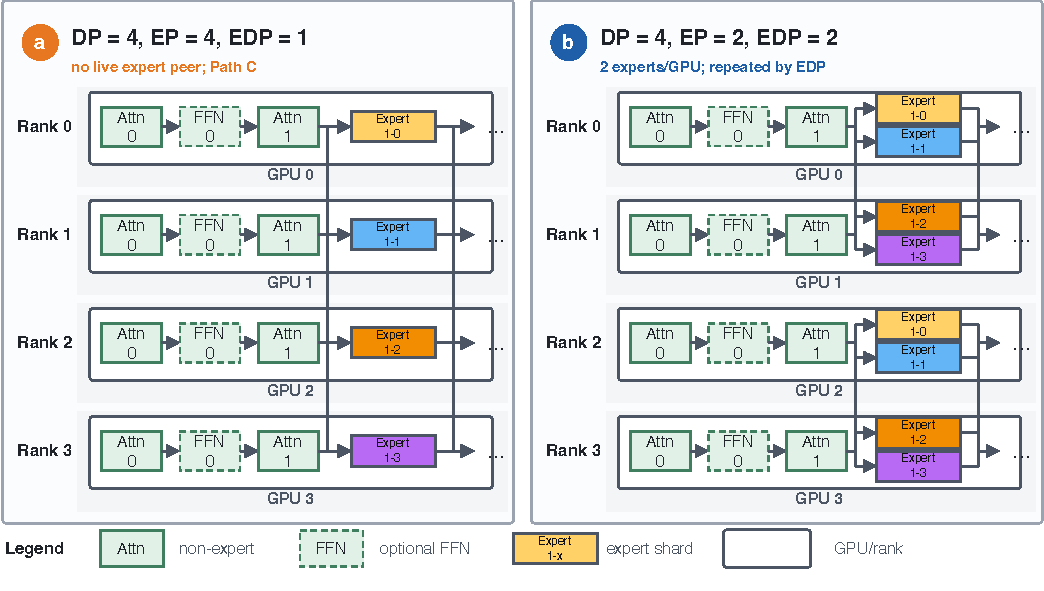
\includegraphics[width=\columnwidth]{edp_distribution.pdf}
\caption{Expert distribution with 8~GPUs (dense TP$=$1, ETP$=$1, PP$=$2). With EDP$>$1, experts have live peers; with EDP$=$1, each expert shard is unique and must be recovered from checkpoint. Non-expert parameters (green) are dense-DP-replicated in both layouts.}
\label{fig:edp-distribution}
\end{figure}

The software-engineering consequence is that \textbf{the same failure invalidates different state classes with different recovery semantics}; standard checkpoint restart does not exploit this boundary.

\subsection{Existing Flow: Checkpoint Restart and the Hidden Risk of Partial Recovery}
\label{sec:bg-flow}

\textbf{Motivating example.} In our 64-GPU Qwen3-30B-A3B job, a failure detected at step $t\!=\!200$ with the latest checkpoint at $c\!=\!100$ causes standard Megatron-LM to reload a 56\,GB distributed checkpoint and replay 100 iterations, for an outage of $\sim$1067\,s. The failed rank, however, owns only 16 of 128 experts; non-expert layers and the other 112 experts remain live on healthy ranks. A MoE-aware recovery path can therefore pull 3.2\,GB of non-expert state from a peer, load only the failed rank's expert shard, and resume from step $t$ in 29\,s with no replay. This opportunity also introduces a quality risk: the recovered experts are stale by $\Delta=t-c$ iterations.

Production LLM training commonly uses \emph{checkpoint restart}~\cite{narayanan2021megatron,dubey2024llama3,jiang2024megascale}: on a failure, the job reloads the most recent globally consistent snapshot at step $c$ and replays the $t-c$ lost iterations. Classical rollback-recovery and checkpoint-interval analyses~\cite{elnozahy2002survey,young1974first,daly2006higher} show that the optimal checkpoint interval scales as $\tau^{*}\!\approx\!\sqrt{2CM}$, where $C$ is the per-checkpoint cost and $M$ is the mean time between failures; with $M$ collapsing to tens of minutes on 10K-GPU clusters~\cite{dubey2024llama3,jiang2024megascale}, repeated failures can consume substantial aggregate GPU-hours in checkpoint I/O and replay.

Restart treats the entire job as a single all-or-nothing state object. Table~\ref{tab:state-provenance} shows why this is wasteful: a single failed rank invalidates only its EP-sharded expert state, while the dense-DP-replicated non-expert state of every other rank at the same PP/dense-TP coordinate remains current at step $t$. A natural alternative is \emph{hybrid recovery}: synchronize non-expert state from a healthy dense-DP peer at the current step, and load only the rank-local experts from the latest checkpoint shard at step $c$. Hybrid recovery, however, introduces a side effect that restart does not: the recovered rank's expert state is stale by $\Delta = t-c$ iterations relative to the rest of the model.

\begin{table}[!t]
\caption{Provenance of MoE training state at iteration $t$ in the EDP$=1$ recovery case.}
\label{tab:state-provenance}
\setlength{\tabcolsep}{1pt}
\renewcommand{\arraystretch}{1.12}
\footnotesize
\begin{center}
\begin{tabular}{@{}lll@{}}
\toprule
\textbf{State} & \textbf{Layout} & \textbf{Source} \\
\midrule
Non-expert (attn/embed/router) & Dense-DP & Peer (step $t$) \\
Expert weights      & EP/ETP & Checkpoint shard ($c\!<\!t$) \\
Expert optimizer    & EP/ETP & Checkpoint shard ($c\!<\!t$) \\
Runtime metadata    & Rank-derived  & Recomputed \\
\bottomrule
\end{tabular}
\end{center}
\end{table}

This staleness is not a binary defect---restored experts still produce valid forward/backward signals---but it can perturb the load-balancing dynamics driven by the MoE auxiliary loss~\cite{shazeer2017outrageously,fedus2022switch,zoph2022stmoe,komatsuzaki2023sparse}. The risk has two dimensions: a \emph{per-event} gap $\Delta$ for the experts owned by the failed rank, and a \emph{window-level} debt accumulated by repeated hybrid recoveries across different expert shards. A recovery system that allows partial repair therefore needs a runtime-checkable bound on accumulated staleness, not only a fast mechanism.


\textbf{Problem statement.} MoEGambit receives a fail-stop event $\langle r,t,c\rangle$ from the cluster watchdog, where $r$ is the failed logical rank, $c$ is the latest checkpoint, and $t$ is the first step that should execute after safe-point handling. If a failure is detected mid-iteration, R1 discards that in-flight iteration and advances $t$ to the next valid step; thus $\Delta=t-c$ counts the iterations that checkpoint restart would replay. MoEGambit must choose either \textsc{Restart}, which restores all state from checkpoint and replays $t-c$ iterations, or \textsc{Hybrid}, which restores current non-expert state from a dense-DP peer and expert state from the failed rank's checkpoint shard. In both cases, the first post-recovery \texttt{optimizer.step()} must be a valid AdamW update: no gradient may be applied to uninitialized or partially restored parameters.

\textbf{Requirements.} We formulate the recovery path as a contract with three software-engineering requirements. \textbf{R1} defines a repair point and gates optimizer commits so a mid-step failure cannot corrupt model state. \textbf{R2} specifies hybrid eligibility through a quantitative, $O(1)$ guard that captures per-event and accumulated staleness. \textbf{R3} records every decision, guard input, latency segment, and state-machine transition for post-hoc auditability. MoEGambit assumes fail-stop rank failures, at least one available checkpoint, a healthy dense-DP peer for the failed rank's non-expert state, and a replacement/hot-spare GPU; if the peer condition fails, the policy chooses \textsc{Restart}.

\section{Approach}
\label{sec:moegambit}

\subsection{Overview}
\label{sec:arch}

MoEGambit is a runtime recovery layer that intercepts rank-failure events and reconstructs the replacement rank's state from the most current available source for each state class, without rolling back the rest of the job. Fig.~\ref{fig:moegambit-overview} summarizes the runtime architecture. The design separates \emph{what is guaranteed} (the recovery contract, R1--R3) from \emph{how state is repaired} (the hybrid restoration mechanism and two-phase protocol), so the contract can be audited independently of the implementation.

\begin{figure*}[!t]
\centering
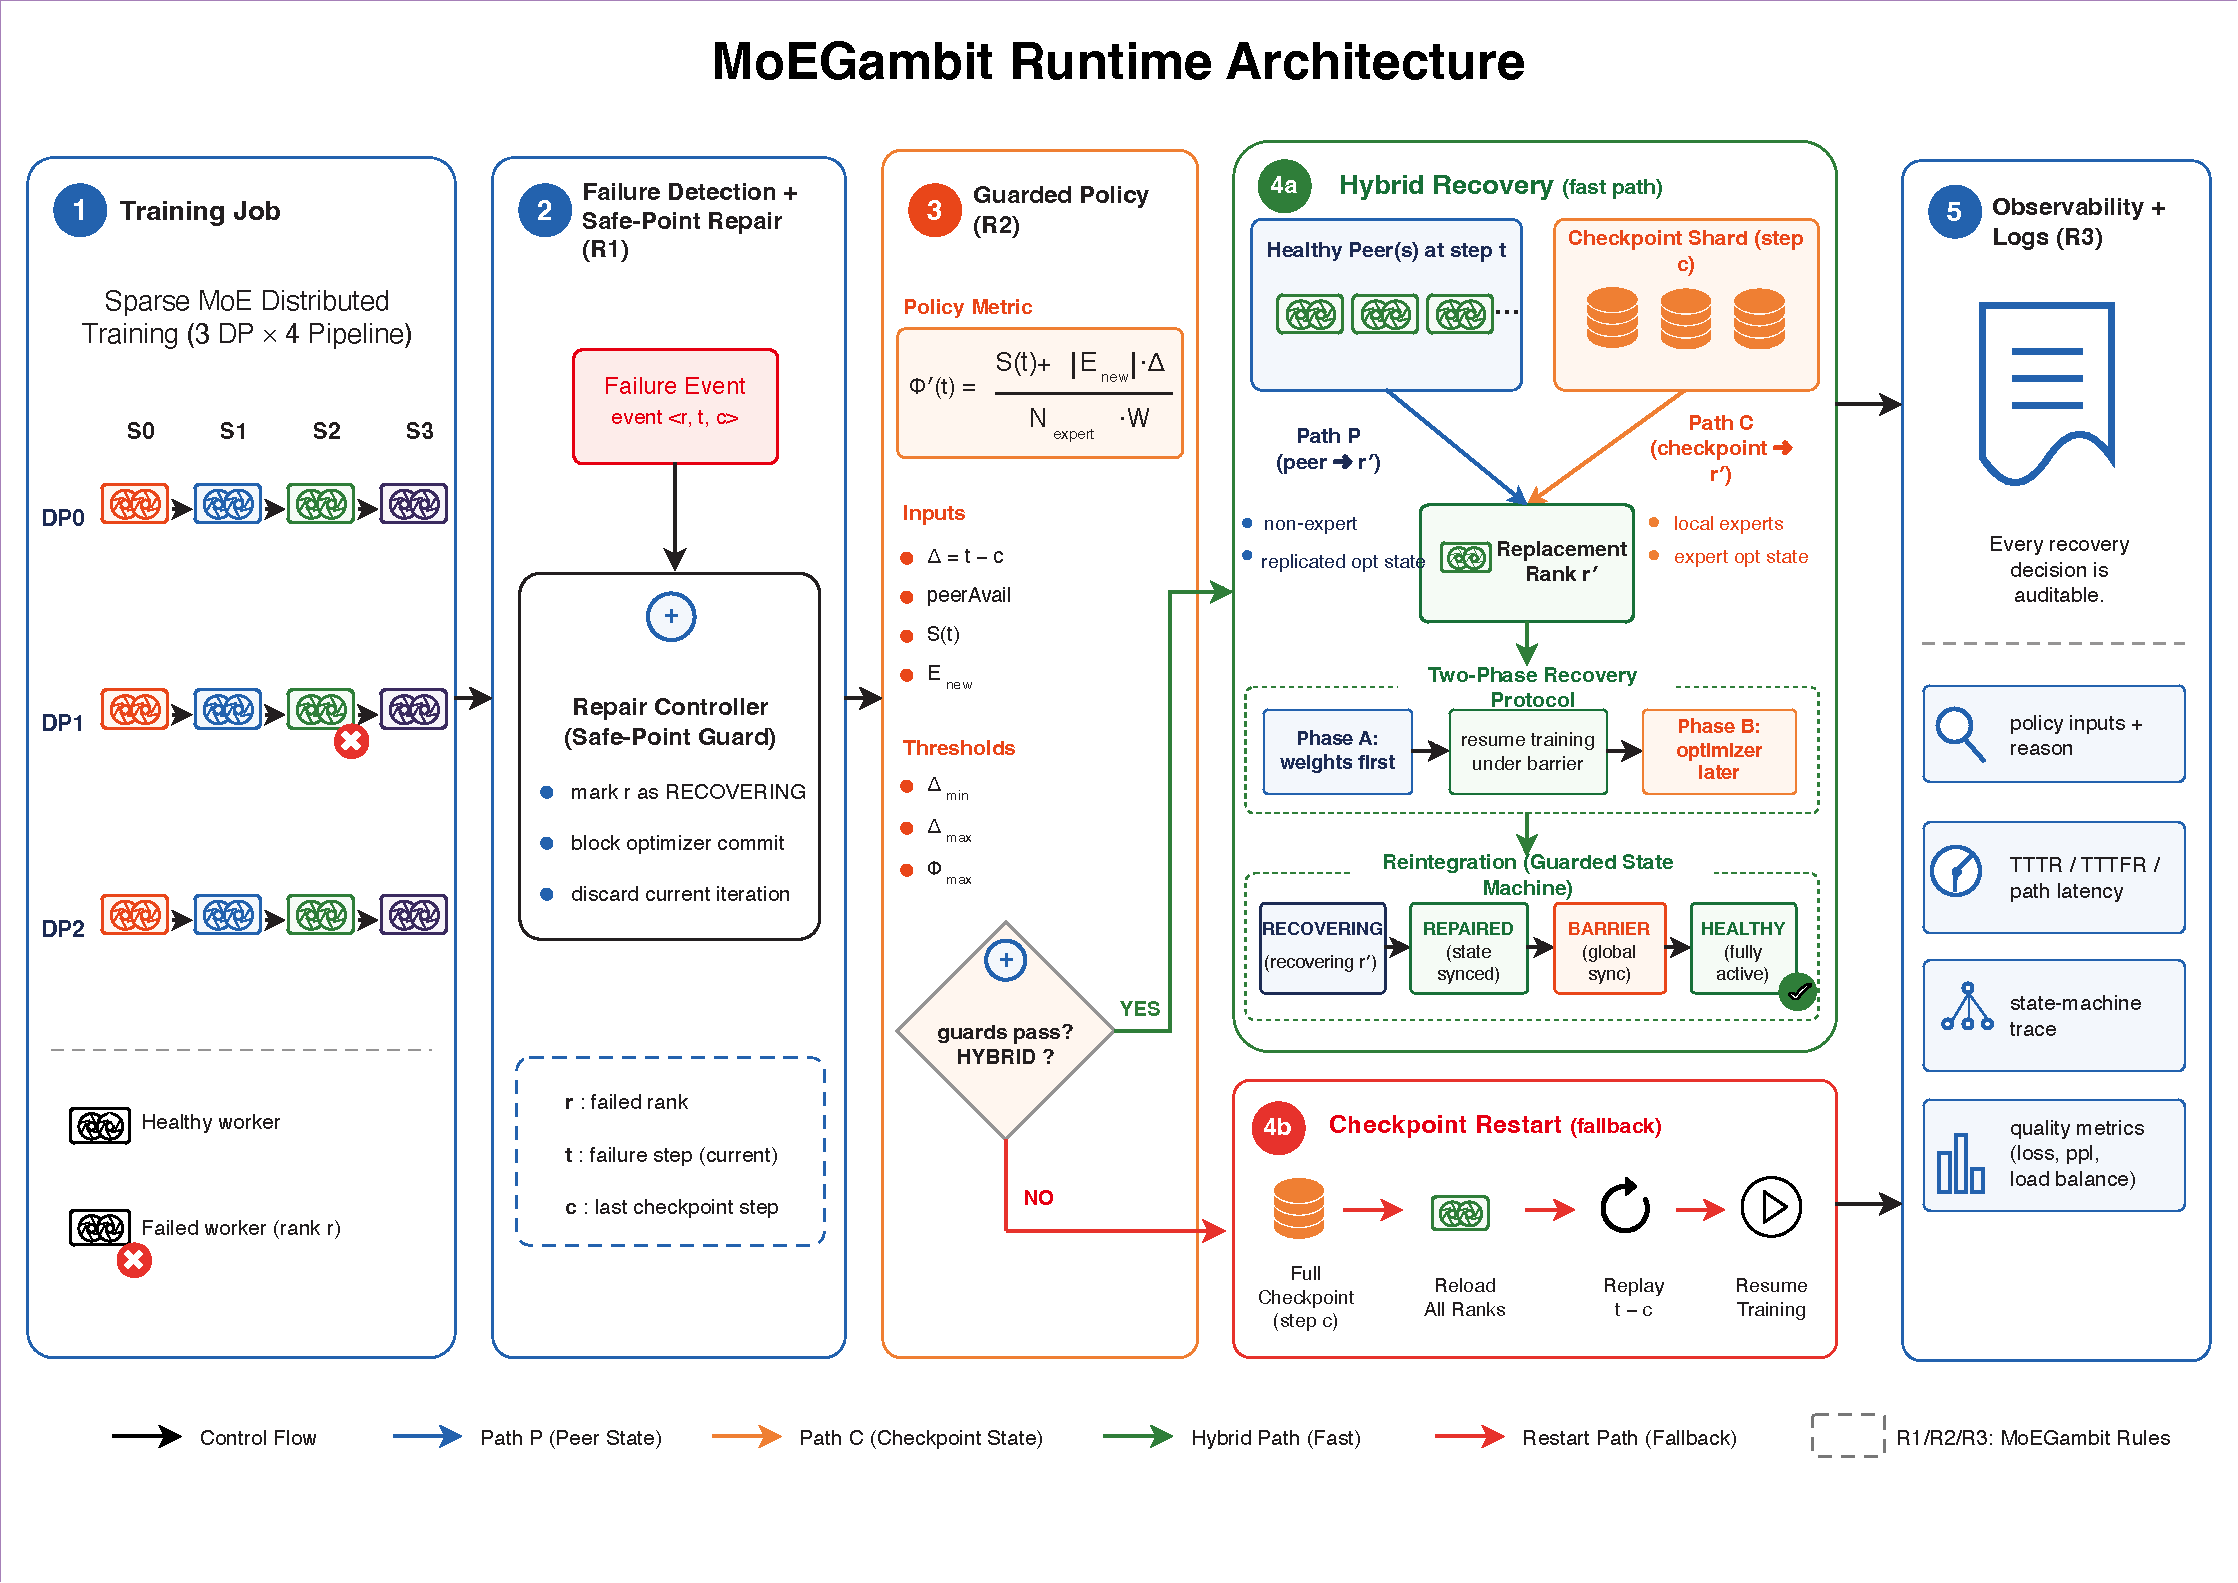
\includegraphics[width=\textwidth]{moegambit_runtime_architecture.pdf}
\caption{MoEGambit runtime architecture. On a rank failure, R1 establishes a repair point, R2 chooses \textsc{Hybrid} or \textsc{Restart}, the hybrid path restores replicated and expert state from different sources, and R3 logs the guarded reintegration trace.}
\label{fig:moegambit-overview}
\end{figure*}

The framework executes five components on each failure event (Fig.~\ref{fig:moegambit-overview}):
\begin{enumerate}
    \item \emph{Failure detection.} An external watchdog emits a failure event $\langle r,t,c\rangle$ identifying the failed rank, the current training step, and the latest checkpoint step.
    \item \emph{Safe-point repair controller} (\S\ref{sec:safepoint}, R1). Installs an optimizer commit guard so no rank applies gradients computed during recovery.
    \item \emph{Staleness-density guarded policy} (\S\ref{sec:policy}, R2). Evaluates the $O(1)$ guard $\Phi'(t)$ and returns a deterministic decision $\pi(t)\!\in\!\{\textsc{Hybrid},\textsc{Restart}\}$. If the projected staleness density exceeds the empirical quality threshold, MoEGambit falls back to checkpoint restart.
    \item \emph{MoE-aware hybrid restoration and two-phase protocol} (\S\ref{sec:mechanism}--\S\ref{sec:twophase}). Pulls non-expert state from a healthy dense-DP peer at step $t$ (path~P), loads rank-local experts from the checkpoint shard at step $c$ (path~C), and overlaps optimizer-state restoration with resumed computation.
    \item \emph{Reintegration state machine and structured logs} (\S\ref{sec:obs}, R3). Advances the replacement rank to \texttt{HEALTHY} and emits a structured record linking policy inputs, latencies, and state-machine transitions.
\end{enumerate}

\subsection{Safe-Point Repair Controller (R1)}
\label{sec:safepoint}

R1 defines a single program point at which repair may run, with one invariant: no optimizer commit may use gradients computed under \texttt{RECOVERING}. On a failure event $\langle r,t,c\rangle$, the controller atomically marks $r$ and its experts as \texttt{RECOVERING}, installs a pre-AdamW commit guard on every rank, and marks the current iteration as \texttt{DISCARD}. Any rank reaching \texttt{optimizer.step()} under \texttt{DISCARD} skips the update; in-flight gradients are dropped. Training then resumes through hybrid repair (\S\ref{sec:mechanism}) or restart, and the controller logs the safe-point status.

\subsection{Staleness-Density Guarded Policy (R2)}
\label{sec:policy}

R2 defines an $O(1)$ guard $\Phi'(t)$ and a deterministic decision $\pi(t)\!\in\!\{\textsc{Hybrid},\textsc{Restart}\}$. The decision uses the failure event $\langle r,t,c\rangle$, the window staleness debt $S(t)=\sum_{h\in\mathcal{H}_{W_{\mathrm{exp}}}(t)}|E_h|\Delta_h$, the predicate $\textsc{PeerAvail}(r,t)$, and thresholds $(\Delta_{\min},\Delta_{\max},\Phi_{\max})$ calibrated in \S\ref{sec:eval}. Here $W_{\mathrm{exp}}$ is the exposure-window length, $\mathcal{H}_{W_{\mathrm{exp}}}(t)$ is the set of previous hybrid events in $[t\!-\!W_{\mathrm{exp}},t)$, $E_h$ is the expert set restored by event $h$, $\Delta_h$ is its checkpoint gap, and $N_{\text{expert}}$ is the routed-expert count in the exposure domain; thus $S(t)$ has units of expert-iterations. If the current event were recovered through the hybrid path, the projected density would be
\begin{equation}
    \label{eq:phi-prime}
    \Phi'(t) \;=\; \frac{S(t) \,+\, |E_{\text{new}}|\, \Delta}{N_{\text{expert}}\cdot W_{\mathrm{exp}}},
\end{equation}
where $N_{\text{expert}}\!\cdot\!W_{\mathrm{exp}}$ is the debt of exposing all experts for one full window; $\Phi'(t)=0.1$ therefore means a projected exposure equal to 10\% of that full-window budget. The value is an exposure density, not a probability, and can exceed 1 under repeated exposure within the window. The running aggregate $S(t)$ is maintained as a single scalar: add $|E_h|\Delta_h$ when a hybrid event $h$ enters the window, and subtract the same product when that event leaves the window (older than $W_{\mathrm{exp}}$ iterations). This yields $O(1)$ per-iteration bookkeeping. When multiple ranks fail simultaneously, each failed rank contributes its own $|E_h|\Delta_h$ term to $S(t)$ before the policy is evaluated for the next rank.

\textbf{Intuition.} The guard is a monitorable exposure budget, not a claim of global convergence. A hybrid event exposes $|E_h|$ experts to weights that are $\Delta_h$ iterations behind the rest of the model; repeated events expose more experts for longer. Charging each event by $|E_h|\Delta_h$ captures both factors, and normalizing by $N_{\text{expert}}\!\cdot\!W_{\mathrm{exp}}$ makes $\Phi'(t)$ comparable across model sizes and window lengths. The threshold $\Phi_{\max}\!=\!10^{-1}$ (\S\ref{sec:eval}) is calibrated against the observed failure-free noise floor.

The decision is
\begin{equation}
    \label{eq:policy}
    \pi(t) \;=\;
    \begin{cases}
        \textsc{Hybrid}, & \text{if } \textsc{PeerAvail}(r,t) \;\wedge\; \\
                         & \quad \Delta_{\min} \leq \Delta \leq \Delta_{\max} \;\wedge\; \\
                         & \quad \Phi'(t) \leq \Phi_{\max}, \\[2pt]
        \textsc{Restart}, & \text{otherwise}.
    \end{cases}
\end{equation}
Algorithm~\ref{alg:policy} encodes the same logic and records the first failing guard on every fallback. The three thresholds play distinct roles. $\Delta_{\min}$ is a cost-benefit lower bound that avoids hybrid repair when the replay gap is too small to offset its coordination cost; $\Delta_{\max}$ is a per-event staleness cap on any single recovered expert shard; and $\Phi_{\max}$ is a window-level cap on accumulated expert exposure. Each threshold is tied to a measurable source: $\Delta_{\min}$ to the $T_{\text{load}}\!:\!T_{\text{hybrid}}\!:\!T_{\text{iter}}$ ratio, $\Delta_{\max}$ to the checkpoint interval bounded by Young/Daly~\cite{young1974first,daly2006higher}, $\Phi_{\max}$ to the guard-disabled quality sweep, and $\textsc{PeerAvail}$ to the live process group. The log entry contains $\langle\pi(t),\text{reason}\rangle$ and $(\Delta,|E_{\text{new}}|,S(t),\Phi'(t))$ (\S\ref{sec:obs}); the compact reason labels identify peer unavailability, the two gap guards, the exposure guard, and the allowed hybrid path.

\begin{algorithm}[!b]
\caption{Guarded recovery decision $\pi(t)$.}
\label{alg:policy}
\begin{algorithmic}[1]
\Require event $\langle r,t,c\rangle$; debt $S(t)$; constants $N_{\text{expert}},W_{\mathrm{exp}}$
\Require guards $(\Delta_{\min},\Delta_{\max},\Phi_{\max})$; \textsc{PeerAvail}
\Ensure recovery decision and first-failing reason
\State $\Delta \gets t-c$; $e \gets |E_{\text{new}}(r)|$
\State $\rho \gets (S(t)+e\Delta)/(N_{\text{expert}}W_{\mathrm{exp}})$
\If{$\neg\,\textsc{PeerAvail}(r,t)$}
    \State \Return $(\textsc{Restart},\textsc{NoPeer})$
\ElsIf{$\Delta < \Delta_{\min}$}
    \State \Return $(\textsc{Restart},\textsc{SmallGap})$
\ElsIf{$\Delta > \Delta_{\max}$}
    \State \Return $(\textsc{Restart},\textsc{LargeGap})$
\ElsIf{$\rho > \Phi_{\max}$}
    \State \Return $(\textsc{Restart},\textsc{HighDebt})$
\Else
    \State \Return $(\textsc{Hybrid},\textsc{Admit})$
\EndIf
\end{algorithmic}
\end{algorithm}

\subsection{Theoretical Rationale for the Guard}
\label{sec:guard-rationale}

The recovery contract is the monitorable admission condition under which MoEGambit may choose the fast path. For every recovery event, hybrid recovery implies all three guards:
\begin{equation}
\label{eq:runtime-contract}
\begin{aligned}
\pi(t)=\textsc{Hybrid} \Rightarrow{}&
\textsc{PeerAvail}(r,t)\\
&{}\wedge\;\Delta_{\min}\leq\Delta\leq\Delta_{\max}\\
&{}\wedge\;\Phi'(t)\leq\Phi_{\max},\quad \forall t.
\end{aligned}
\end{equation}
R3 logs evidence for each conjunct, so the contract is checkable online and auditable offline. The threshold $\Phi_{\max}$ is empirical, but the form of $\Phi'(t)$ follows from a first-order exposure bound.

\noindent\textbf{Proposition 1 (expert-exposure bound).}
Let $\theta_e(s)$ denote expert $e$'s state after step $s$. Assume that, within a recovery window and with non-expert state fixed, the monitored MoE loss component $\ell_{\text{aux}}$ is coordinate-wise $L_{\text{aux}}$-Lipschitz in each expert state, and a normal step changes any expert by at most $G$ in the same norm. If event $h$ restores expert set $E_h$ from checkpoint step $c_h$ and resumes at $t_h$, then its stale-expert perturbation relative to a current-state restore satisfies
$\delta\ell_h \leq L_{\text{aux}}\sum_{e\in E_h}\|\theta_e(t_h)-\theta_e(c_h)\| \leq L_{\text{aux}}G\,|E_h|\,(t_h-c_h)$.
Consequently, after adding the current candidate event to the existing window debt,
$\sum_{h\in\mathcal{H}_{W_{\mathrm{exp}}}(t)\cup\{\text{new}\}}\delta\ell_h \leq L_{\text{aux}}G\,(S(t)+|E_{\text{new}}|\Delta)=L_{\text{aux}}G\,N_{\text{expert}}W_{\mathrm{exp}}\Phi'(t)$.
Thus $\Phi'(t)$ is a normalized exposure proxy whose induced first-order perturbation bound scales linearly with $\Phi'(t)$; it is not a standalone convergence theorem.

\subsection{MoE-Aware Hybrid State Restoration}
\label{sec:mechanism}

When $\pi(t)=\textsc{Hybrid}$, the replacement rank reconstructs its state by reading each state class from its most current available source (Table~\ref{tab:state-provenance}), so I/O scales with the rank-unique expert volume rather than the full distributed checkpoint. Two paths run concurrently. \emph{Path~P (peer pull, replicated state)} synchronizes current-step non-expert parameters (and dense-DP-replicated optimizer state) from a healthy peer at the same PP/dense-TP coordinate via a single P2P broadcast over NCCL/Gloo; the transfer completes in tens of milliseconds. \emph{Path~C (shard read, sharded expert state)} loads rank-$r$'s experts from the per-rank shard at step $c$ with no collectives. The recovered rank is intentionally mixed: non-expert state reflects step $t$, while experts and their optimizer state are stale by $\Delta$---the quantity bounded by $\Phi'(t)$ in (\ref{eq:phi-prime}) (Fig.~\ref{fig:moegambit-overview}, step 4a).

\subsection{Two-Phase Recovery Protocol}
\label{sec:twophase}

The two-phase protocol reduces time-to-resume by overlapping path~C's optimizer-state read with resumed forward/backward, while forbidding commits on uninitialized expert slots. \emph{Phase~A (weights first)} restores non-expert state and expert weights, then rejoins under an \emph{update barrier}: forward/backward contributes to the global loss, but gradients for affected experts are buffered. \emph{Phase~B (optimizer later)} restores non-expert and expert moments in parallel; when it completes, the barrier releases and buffered gradients are applied via one AdamW step. The barrier reuses the pre-\texttt{step()} hook of \S\ref{sec:safepoint}, so R1 holds throughout. The log records $T_{\text{TTR}}$ and $T_{\text{TTFR}}$; their gap is the latency saved over single-phase restart. Because the protocol controls \emph{when} optimizer state attaches, not \emph{where} bytes come from, \S\ref{sec:rq1}'s $2{\times}2$ factorial tests it independently of hybrid restore.

\subsection{Reintegration State Machine and Structured Logs (R3)}
\label{sec:obs}

R3 requires that every recovery decision and its downstream model-quality outcome be traceable. We implement R3 through two mechanisms: a guarded state machine that enforces the reintegration protocol, and a structured log that records the inputs and outputs of each recovery event.

\textbf{Guarded state machine.} Each replacement rank advances through a four-state linear protocol:
\begin{equation}
\label{eq:state-machine}
\texttt{RECOVERING} \xrightarrow{g_1} \texttt{REPAIRED} \xrightarrow{g_2} \texttt{BARRIER} \xrightarrow{g_3} \texttt{HEALTHY},
\end{equation}
where each transition is gated by a guard predicate:
\begin{itemize}
    \item $g_1$: state restoration complete---all state classes (non-expert via path~P, experts via path~C) have been loaded and verified against their source checksums.
    \item $g_2$: dispatch topology re-derived---the expert directory and all-to-all routing tables have been recomputed to reflect the replacement rank's position in the EP layout.
    \item $g_3$: optimizer state attached and update barrier released---Phase~B of the two-phase protocol (\S\ref{sec:twophase}) has completed, and the buffered gradients have been applied.
\end{itemize}
Because every transition requires its guard to hold, the state machine rejects premature reintegration---e.g., routing tokens to an expert whose optimizer state has not yet been restored.

\textbf{Structured recovery log.} On each recovery event, the state machine emits one record with policy inputs ($\Delta$, $|E_{\text{new}}|$, $S(t)$, $\Phi'(t)$), the decision and reason string, per-segment latencies, and transition timestamps. This record links every recovery path back to the guards in (\ref{eq:policy}) and supports post-hoc correlation with training-quality metrics under the paired-run methodology of \S\ref{sec:eval}~\cite{wohlin2012ese,arcuri2014hitchhiker}. The overhead of $\Phi'(t)$ accounting and log emission is $O(1)$ per iteration and empirically negligible (\S\ref{sec:rq4}).

\subsection{Implementation}
\label{sec:impl}

MoEGambit is implemented as a Python extension to Megatron-LM (commit \texttt{core\_r0.9.0}) covering safe-point control, policy evaluation, hybrid restore, two-phase optimizer recovery, and reintegration. It hooks optimizer-step, checkpoint-load, and collective paths while preserving standard checkpoint restart; without \texttt{-{}-enable-moegambit}, training follows the standard path. The anonymized supplementary material contains the full system code, structured logs, and plotting/reproduction scripts; we will make the artifacts public after the double-anonymous review period.



\section{Evaluation}
\label{sec:eval}

This section evaluates whether MoEGambit reduces recovery cost without degrading the post-recovery training trajectory. We ask six research questions:

\begin{itemize}
    \item \textbf{RQ1:} How much recovery cost does MoEGambit reduce, and do hybrid restore and two-phase recovery compose additively?
    \item \textbf{RQ2:} Does hybrid recovery permitted by the contract avoid detectable quality degradation relative to failure-free training?
    \item \textbf{RQ3:} Does $\Phi'(t)$ separate low-exposure recoveries from risky repeated and burst failures?
    \item \textbf{RQ4:} What overhead do the monitoring hooks add during failure-free training?
    \item \textbf{RQ5:} Does the recovery advantage hold across scale and parallelism layouts?
    \item \textbf{RQ6:} Does the mechanism generalize to a different MoE model configuration?
\end{itemize}

\subsection{Experimental Setup}

\textbf{Cluster and parallelism.} Unless otherwise stated, experiments ran on 64 H20-3e GPUs (8 nodes $\times$ 8 GPUs) with dense TP$=1$, PP$=8$, EP$=8$, ETP$=1$, and EDP$=1$ under the Megatron Core definition. The scalability and parallelism-sensitivity experiments used the overrides described in RQ5.

\textbf{Model and tokenizer.} We used \emph{Qwen3-30B-A3B}~\cite{qwen3report} (30B total / 3B activated, 48 layers, 128 experts, top-8 routing) with the Qwen2Tokenizer (151{,}936-token byte-level BPE). Default training hyperparameters are in Table~\ref{tab:config}.

\begin{table}[!b]
\caption{Default training configuration.}
\begin{center}
\footnotesize
\setlength{\tabcolsep}{3pt}
\begin{tabular}{@{}llll@{}}
\toprule
\textbf{Parameter} & \textbf{Value} & \textbf{Parameter} & \textbf{Value} \\
\midrule
Layers & 48 & Experts & 128 \\
Hidden size & 2048 & MoE top-$k$ & 8 \\
Attention heads & 32 & MoE FFN hidden & 768 \\
Query groups & 4 & Load balancing & aux. loss \\
Sequence length & 4096 & Aux. coef. & $1 \times 10^{-3}$ \\
Global batch & 64 & Optimizer & AdamW \\
Precision & BF16 & LR/min LR & $10^{-4}/10^{-5}$ \\
LR schedule & cosine & Weight decay & 0.1 \\
Gradient clipping & 1.0 & & \\
\bottomrule
\end{tabular}
\label{tab:config}
\end{center}
\end{table}

\textbf{Data.} We used a 4B-token subset of \emph{FineWeb}~\cite{penedo2024fineweb}, processed into Megatron indexed format. We used a held-out validation split for loss/perplexity reported every 1{,}000 iterations. All recovery experiments used \emph{paired runs}: baseline and MoEGambit shared the same seed, data order, checkpoint, and injected failure step.

\textbf{Baseline timing and noise scale.} Steady-state $T_{\text{iter}}\!\approx\!10.31$\,s; full-checkpoint load $T_{\text{load}}\!\approx\!35.95$\,s; hybrid recovery $T_{\text{hybrid}}\!\approx\!28.91$\,s; \texttt{save-interval}$=200$ (Young/Daly optimal~\cite{young1974first,daly2006higher}). Ten NoFault runs yielded $\mu_{\text{base}}=4.8543$, $\sigma_{\text{base}}=0.024$ on iter-600 eval loss; we used $\sigma_{\text{base}}$ to scale deviations and reported both $\pm1\sigma_{\text{base}}$ and $\pm2\sigma_{\text{base}}$ bands. This noise scale captures residual variation from collective-communication timing, node/GPU heterogeneity, shared-storage jitter, and nondeterministic kernel scheduling that remains even with fixed seeds and data order.

\textbf{Metrics.} Raw recovery latency excludes replay and ends when the replacement rank reaches \texttt{HEALTHY}; time-to-resume ($T_{\text{TTR}}$) ends at the first valid post-recovery forward pass; time-to-full-recovery ($T_{\text{TTFR}}$) ends when optimizer state is attached and the update barrier is released. End-to-end recovery additionally includes replay for Restart and MoC-System; MoEGambit's hybrid path resumes at step $t$ and has zero replay cost.

\textbf{Statistical treatment.} Latency experiments reported the mean over 500 injected recovery events because recovery cost is dominated by deterministic I/O and collective-transfer segments; quality experiments used paired comparisons to control for seed and data-order noise. We used NoFault $\sigma_{\text{base}}$ bands as practical effect-size references and paired nonparametric tests to assess degradation; we did not require every individual recovered run to lie inside the $\pm1\sigma_{\text{base}}$ band.

\subsection{Compared Systems}\label{sec:compared}

We compared MoEGambit with three baselines: \textbf{NoFault} (no injected failures, reference trajectory); \textbf{Restart} (standard Megatron-LM checkpoint restart with full reload and replay); and \textbf{MoC-System} (a published MoE-specific baseline with enough detail for timing and quality reproduction~\cite{cai2024moc}). We discuss MoEvement~\cite{gandhi2026moevement} in Related Work because it relies on sparse checkpointing plus activation/gradient logging, whereas MoEGambit uses peer-current non-expert repair without logging intermediate activations or gradients.

\textbf{MoC-System.} MoC-System is a save-side MoE fault-tolerance system that reduces checkpointing cost with Partial Experts Checkpointing (PEC): each checkpoint stores only a selected subset of experts and rotates that subset across saves. Because no public reference implementation is available, we separated accuracy and timing. For accuracy, we reproduced the best PEC configuration reported in the MoC-System paper ($K_{\text{pec}}=16$, $N=128$, PLT~$\approx 3.75\%$) by redirecting each non-fresh expert to its corresponding historical checkpoint shard, with MoEGambit's hybrid repair and two-phase protocol disabled. For timing, we used the best recovery numbers reported by, or derivable from, the paper; since MoC-System is save-side, recovery still resumes from checkpoint state and replays lost iterations to reach step $t$.

\subsection{Policy Parameters}

MoEGambit uses three thresholds: $\Delta_{\min}$, $\Delta_{\max}$, $\Phi_{\max}$ (Table~\ref{tab:policy}).

\begin{table}[!b]
\caption{Default policy parameters.}
\label{tab:policy}
\setlength{\tabcolsep}{4pt}
\renewcommand{\arraystretch}{1.1}
\begin{center}
\begin{tabular}{@{}l p{0.46\columnwidth} l@{}}
\toprule
\textbf{Param.} & \textbf{Meaning} & \textbf{Default} \\
\midrule
$\Delta_{\min}$    & Min. gap for hybrid recovery                         & 1\,iter           \\
$\Delta_{\max}$    & Max. single-event gap for hybrid recovery            & 200\,iters        \\
$\Phi_{\max}$      & Max. staleness density in $W_{\mathrm{exp}}$          & $1\!\times\!10^{-1}$ \\
$W_{\mathrm{exp}}$ & exposure window                                       & 2\,000\,iters     \\
$N_{\text{expert}}$ & routed experts in exposure domain                    & 128               \\
\bottomrule
\end{tabular}
\end{center}
\end{table}

$\Delta_{\min}$ and $\Delta_{\max}$ were non-binding under our timings ($T_{\text{load}}>1.2\,T_{\text{hybrid}}$, so hybrid has lower latency for every $\Delta\!\geq\!1$); we retain both as defensive guards for clusters with much faster checkpoint loading.

\textbf{$\Phi_{\max}=10^{-1}$ calibration.} We calibrated the threshold with a guard-disabled $3\!\times\!4$ multi-rank burst sweep (Table~\ref{tab:multi_fault}) to identify the quality-degradation boundary that the default policy should avoid. We set $W_{\mathrm{exp}}=2{,}000$ to cover the 1{,}000-iteration warmup and 1{,}000-iteration post-recovery horizon used in the stability experiment. Under this window, the seven cell means with $\Phi'(t)\!\leq\!10^{-1}$ remained within the baseline $\pm 1\sigma_{\text{base}}$ band, whereas the five cells above the threshold deviated by $1.21$--$1.98\sigma_{\text{base}}$ under always-hybrid recovery. The default policy therefore routes those five over-threshold cells to checkpoint restart.

\begin{table}[!t]
\caption{Guard-disabled burst sweep: validation-loss deviation under always-hybrid recovery (units of $\sigma_{\text{base}}$). Shaded cells exceed $\Phi_{\max}$ and trigger restart under the default policy.}
\label{tab:multi_fault}
\setlength{\tabcolsep}{6pt}
\renewcommand{\arraystretch}{1.1}
\begin{center}
\footnotesize
\begin{tabular}{@{}r|cccc@{}}
\toprule
$|F|$ & $\Delta\!=\!50$ & $\Delta\!=\!100$ & $\Delta\!=\!150$ & $\Delta\!=\!200$ \\
\midrule
$8$  & $+0.32$ & $+0.64$ & $-0.05$ & $+0.01$ \\
$16$ & $-0.18$ & $+0.71$ & \cellcolor{red!12}$+1.42$ & \cellcolor{red!12}$+1.46$ \\
$24$ & $+0.59$ & \cellcolor{red!12}$+1.21$ & \cellcolor{red!12}$+1.98$ & \cellcolor{red!12}$+1.95$ \\
\bottomrule
\end{tabular}
\end{center}
\end{table}

\subsection{RQ1: Single-Failure Recovery Cost and Mechanism Decomposition}
\label{sec:rq1}

RQ1 measures the low-latency recovery path: how much latency MoEGambit saves and whether its two mechanisms compose independently.

We injected hard failures after warmup and ran a $2\times 2$ factorial crossing \textbf{(i)~hybrid restore} versus \textbf{full checkpoint restart} with \textbf{(ii)~two-phase} versus \textbf{single-phase} optimizer attachment. Each cell aggregated 500 injected recovery events; Table~\ref{tab:single} reports the mean. We measured latency from failure detection until the replacement rank produced its first post-recovery iteration.

\begin{table}[!b]
\caption{Single-failure time-to-resume ($2{\times}2$ factorial; mean per event, seconds, excludes replay).}
\label{tab:single}
\setlength{\tabcolsep}{3pt}
\renewcommand{\arraystretch}{1.15}
\begin{center}
\footnotesize
\begin{tabular}{@{}l r r r@{}}
\toprule
\textbf{Restore path} & \textbf{Single} & \textbf{Two-phase} & \textbf{$\Delta$ (s)} \\
\midrule
Full checkpoint  & 36.417 & 34.238          & $-2.179$ \\
Hybrid (selective) & 30.743 & \textbf{28.914} & $-1.829$ \\
\midrule
$\Delta$ hybrid (s) & $-5.674$ & $-5.324$ & \\
\bottomrule
\end{tabular}
\end{center}
\end{table}

\textbf{Decomposition.} The \emph{hybrid restore} main effect was $-5.50$\,s ($-15.1\%$) and the \emph{two-phase} main effect was $-2.00$\,s ($-5.5\%$), with an interaction of $0.35$\,s ($0.96\%$ of baseline, within noise). The two mechanisms were nearly additive in this experiment, jointly yielding the $28.914$\,s best cell---a \textbf{$20.6\%$ reduction} over full checkpoint restart.

\textbf{Result.} Hybrid restore replaces NVMe-bound full-tensor restoration with peer-pulled non-expert state plus one expert-shard read, reducing I/O from $O(\text{global checkpoint})$ to $O(|E_{\text{new}}|\!\cdot\!\text{shard})$. Two-phase recovery overlaps optimizer-state restoration with resumed forward/backward; in our measurements, this overlap saved a nearly constant $\approx 2$\,s. The small interaction ($0.96\%$) indicated that the mechanisms target different recovery segments.

Because Restart and MoC-System resume from checkpoint state, both replay the expected gap $\Delta\!=\!100$ iterations to reach step $t$ ($T_{\text{replay}}\!\approx\!1031$\,s). Using the best-case load cost above, the replay-inclusive cost was $1067.4$\,s; MoEGambit resumed at step $t$ directly, giving $1067.4/28.9=\mathbf{36.9\times}$ replay-inclusive speedup for this 100-iteration gap. We report raw and replay-inclusive metrics separately; only the latter scales with the replay gap.

\subsection{RQ2: Training Quality and Stability}
\label{sec:rq2}

RQ2 tests the quality side of the recovery contract: does hybrid recovery permitted by the contract avoid detectable degradation relative to failure-free training?

\textbf{Setup.} Each run performed 1{,}000 warmup iterations, injected one failure, and then continued for 1{,}000 iterations against paired NoFault and Restart runs. Gaps that satisfied the contract ($\Delta\!\in\!\{64,128\}$) used the hybrid path; larger forced gaps $\Delta\!\in\!\{256,512,1000,1500\}$ stressed the per-event guard and routed to restart unless the guard was deliberately disabled.

\textbf{Result.} For tested contract-satisfying hybrid gaps, paired validation loss and perplexity showed \textbf{no statistically detectable degradation} relative to NoFault/Restart. Fig.~\ref{fig:train-loss} shows the full 10{,}000-iteration trajectory under ten injected faults, and Fig.~\ref{fig:fault-heatmap} zooms into 50 single-failure runs around the NoFault mean that satisfied the contract: \textbf{44/50} runs fell within $\pm2\sigma_{\text{base}}$ and 23/50 within $\pm1\sigma_{\text{base}}$. A Wilcoxon signed-rank test on the 10 paired eval-loss differences at iter~600 yielded $p\!=\!0.63$ and Cliff's delta $=0.07$, giving no evidence of degradation. We used larger forced gaps only as guard stress tests; under the default policy, those cases route to restart.

Because runs are paired by seed, data order, checkpoint, and failure time, the criterion is conservative: MoEGambit is judged by paired deviation from the baseline trajectory, not by whether a single noisy run improves a score.

\begin{figure}[!t]
\centering
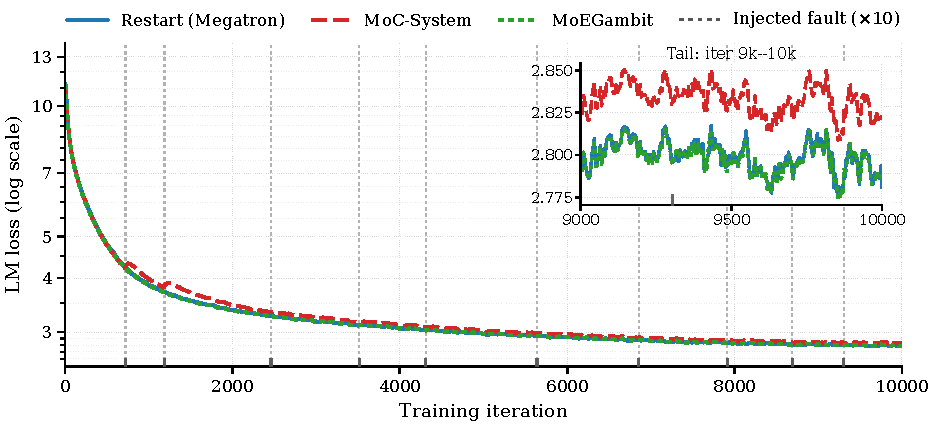
\includegraphics[width=0.98\columnwidth]{train_loss.pdf}
\caption{Training-loss trajectories over 10{,}000 iterations with ten injected faults (gray verticals). Last-200-iteration mean: Restart 2.7919, MoEGambit 2.7910, MoC-System 2.8254.}
\label{fig:train-loss}
\end{figure}

\begin{figure}[!t]
\centering
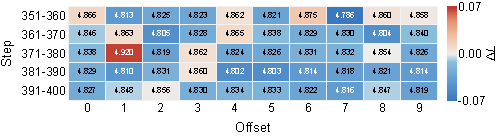
\includegraphics[width=\columnwidth]{fault_heatmap_compact.pdf}
\caption{Eval-loss heatmap for 50 single-failure recoveries that satisfied the contract. Each cell is one run; color encodes deviation from the 10-run NoFault mean ($\mu_{\text{base}}=4.8543$, $\sigma_{\text{base}}=0.024$). The distribution is centered near the baseline, with 44/50 cells within $\pm2\sigma_{\text{base}}$ and 23/50 within $\pm1\sigma_{\text{base}}$.}
\label{fig:fault-heatmap}
\end{figure}

The heatmap targets isolated rank/GPU faults, a common production case emphasized by LLM traces and resilient-training systems~\cite{dubey2024llama3,jiang2024megascale,jang2023oobleck}. As larger jobs increase EP or shard experts more finely, one failed GPU owns a smaller expert fraction, so $\Phi'(t)$ charges less per-event exposure; RQ3 covers bursts whose accumulated exposure triggers fallback.

Across all 10{,}000 iterations and injected faults, MoEGambit tracked Restart within run-to-run noise; MoC-System accumulated a small persistent gap consistent with PEC carrying older expert state across recovery boundaries.

\textbf{Downstream zero-shot accuracy.} Table~\ref{tab:downstream} reports lm-evaluation-harness~\cite{eval-harness} results at iter~10{,}000 on eight tasks (ARC-Easy~\cite{clark2018arc}, BoolQ~\cite{clark2019boolq}, MathQA~\cite{amini2019mathqa}, OpenBookQA~\cite{mihaylov2018obqa}, PIQA~\cite{bisk2020piqa}, RACE~\cite{lai2017race}, SWAG~\cite{zellers2018swag}, WinoGrande~\cite{sakaguchi2020winogrande}).

\begin{table*}[!t]
\caption{Zero-shot downstream accuracy (\%) at iter $10{,}000$ (lm-evaluation-harness; standard errors $\leq 0.021$).}
\label{tab:downstream}
\setlength{\tabcolsep}{5pt}
\renewcommand{\arraystretch}{1.15}
\begin{center}
\small
\begin{tabular}{@{}l ccccccccc@{}}
\toprule
\textbf{System} & \textbf{ARC-E} & \textbf{BoolQ} & \textbf{MathQA} & \textbf{OBQA} & \textbf{PIQA} & \textbf{RACE} & \textbf{SWAG} & \textbf{WG} & \textbf{Avg.} \\
                & acc            & acc            & n               & n             & n             & acc           & n             & acc          &              \\
\midrule
Restart (Megatron)            & 46.72          & 59.88          & 22.08          & 29.00          & \textbf{68.34} & 29.00          & 55.17          & 50.28          & 45.06 \\
MoC-System~\cite{cai2024moc}  & 45.41          & \textbf{59.94} & \textbf{22.28} & 28.20          & 67.68          & 29.19          & 54.00          & \textbf{50.67} & 44.67 \\
MoEGambit                     & \textbf{48.36} & 58.56          & 21.54          & \textbf{30.60} & 68.17          & \textbf{29.28} & \textbf{55.43} & 50.59          & \textbf{45.32} \\
\bottomrule
\end{tabular}\\[2pt]
{\footnotesize\raggedright \textsuperscript{*}\,Per-column best is in \textbf{bold}. Metric row: ``n'' denotes \texttt{acc\_norm}; others are \texttt{acc}.\par}
\end{center}
\end{table*}

Restart and MoEGambit agreed within $\pm 1.6$~pp on every task. MoEGambit was numerically higher on average ($+0.26$~pp), but the gap was inside the per-checkpoint downstream noise floor~\cite{biderman2023pythia}; we interpret it as \textbf{quality parity}. The small positive mean could reflect evaluation noise or mild dropout-like noise regularization from a bounded perturbation to a small expert subset~\cite{srivastava2014dropout,bishop1995noise}. This interpretation is consistent with ST-MoE fine-tuning ablations where updating only non-MoE parameters performs comparably to updating all parameters, while sparse models tolerate some dropped-token noise~\cite{zoph2022stmoe}. It is \textbf{not evidence of improvement}. MoC-System reached $44.67$~\% (\,$-0.39$~pp vs.\ Restart) and trailed on six of eight probes, consistent with the persistent loss gap in Fig.~\ref{fig:train-loss}.

\subsection{RQ3: Multiple Failures and Expert-Weighted Staleness Density}
\label{sec:rq3}

RQ3 stress-tests the R2 specification: does the $\Phi'(t)\!\leq\!\Phi_{\max}$ guard separate low-exposure recoveries from higher-risk multi-rank bursts?

We stress-tested MoEGambit against the calibrated $\Phi_{\max}=10^{-1}$ threshold using repeated and multi-rank burst failures. With \texttt{find\_multi\_fault.sh}, we swept $|F|\!\in\!\{8,16,24\}$ and $\Delta\!\in\!\{50,100,150,200\}$ on the same $3\!\times\!4$ grid as Table~\ref{tab:multi_fault}, plus repeated-window traces that revisit one rank within $W_{\mathrm{exp}}$. This is a calibrated stress test, not an independent proof of generalization.

\textbf{Result.} Under the default policy, MoEGambit used hybrid recovery for the seven $\Phi'(t)\!\leq\!10^{-1}$ cells and redirected the five over-threshold cells to checkpoint restart, where cell-mean loss returned inside the $\pm 1\sigma_{\text{base}}$ band. With the guard disabled, those same five cells reproduced the $1.21$--$1.98\sigma_{\text{base}}$ deviations in Table~\ref{tab:multi_fault}. Thus, the absence of above-threshold degradation came from fallback, and the expert-weighted window captured risk missed by gap-only policies.

This also explains why $\Delta_{\max}$ alone is insufficient: equal-gap events can expose different expert fractions depending on failed ranks and recent repairs. $\Phi'(t)$ charges both gap and affected expert set, then ages the charge out of the window, separating isolated single-rank failures from dense bursts.

\subsection{RQ4: Failure-Free Overhead}
\label{sec:rq4}

\textbf{Result.} Over 1{,}000 failure-free iterations, MoEGambit's hooks added \textbf{$<6$\,\textmu s} per iteration and changed mean step time by only \textbf{$+0.1\%$}; a paired $t$-test did not reject a zero mean difference at $\alpha=0.05$.

\subsection{RQ5: Scalability}\label{sec:rq5}

We reran the single-failure injection of \S\ref{sec:rq1} at 64 and 128 GPUs (dense TP$=$1, PP$=$8, EP$\in\{$8,16$\}$, ETP$=$1; 10 seeds each) and tested four 64-GPU layouts spanning dense TP$\in\{1,2\}$, ETP$\in\{1,2\}$, PP$\in\{4,8\}$, EP$\in\{4,8\}$, and EDP$\in\{1,2\}$. \textbf{Result.} Restart grew with global checkpoint size ($36.4$\,s $\to 47.2$\,s), while MoEGambit grew more slowly ($28.9$\,s $\to 33.7$\,s) because hybrid I/O scales with the per-rank shard. The ratio widened from $1.26\times$ to $\mathbf{1.40\times}$ (Fig.~\ref{fig:scalability}), suggesting larger benefits at larger GPU scales.

\begin{figure}[!t]
\centering
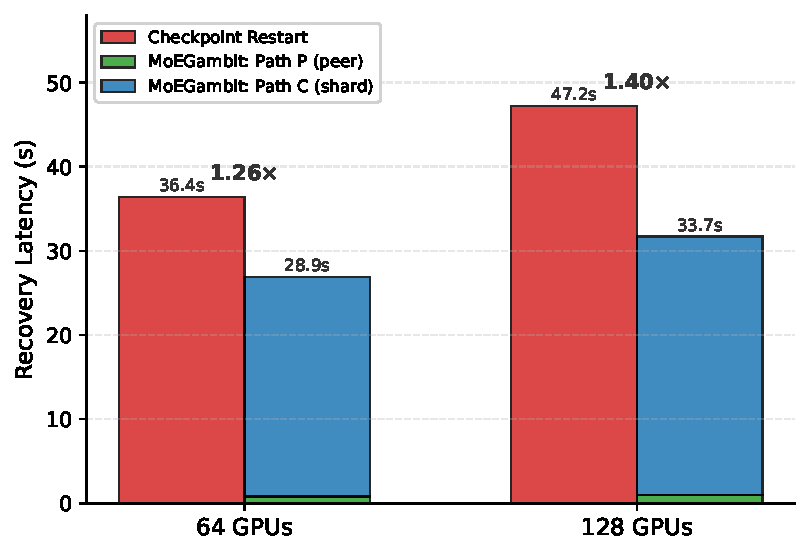
\includegraphics[width=0.60\columnwidth]{scalability.pdf}
\caption{Recovery latency at 64 and 128 GPUs. The Restart/MoEGambit ratio widened from $1.26\times$ to $1.40\times$ because hybrid I/O scales with the per-rank shard.}
\label{fig:scalability}
\end{figure}

\textbf{Parallelism sensitivity.} Across four 64-GPU layouts (Fig.~\ref{fig:par_sensitivity}), MoEGambit outperformed restart by \textbf{$1.26$--$3.56\times$}. The advantage was largest when EDP$\geq$2 because a live expert peer lets MoEGambit restore both non-expert and expert state from peers; even at EDP$=1$, hybrid recovery remained faster by reading only the failed rank's expert shard from disk.

\begin{figure}[!t]
\centering
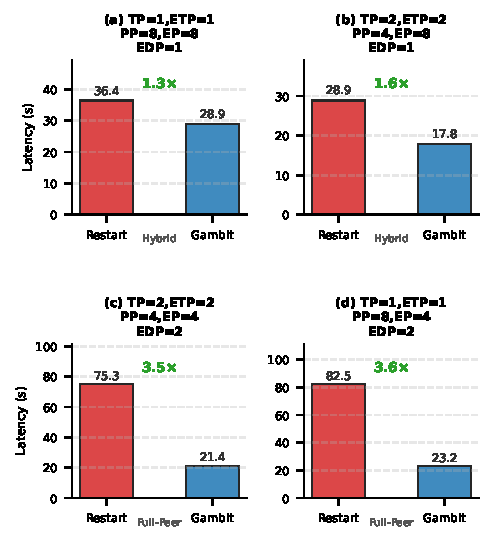
\includegraphics[width=0.60\columnwidth]{parallelism_sensitivity.pdf}
\caption{Parallelism sensitivity at 64~GPUs using the Megatron Core EDP definition. EDP$=$1 layouts used hybrid recovery ($1.26$--$1.62\times$); EDP$=$2 enabled full-peer recovery and yielded $3.52$--$3.56\times$ speedups.}
\label{fig:par_sensitivity}
\end{figure}

\subsection{RQ6: Cross-Model Generalization}\label{sec:rq6}

To assess generalization beyond Qwen3-30B-A3B, we reran the core experiments on \textbf{DeepSeek-V2-Lite}~\cite{deepseekv2} (15.7B total / 2.4B activated, 64 routed experts, 2 shared experts, top-6). Shared experts are dense-DP-replicated and used path~P; routed experts used path~C. Policy parameters were inherited from Table~\ref{tab:policy} with $N_{\text{expert}}\!=\!64$.

\textbf{Result.} Restart took $26.09$\,s while MoEGambit recovered in $11.73$\,s, a \textbf{$55.0\%$ reduction ($2.22\times$)}. Smaller expert shards made path~C faster; the same burst-sweep grid did not require retuning $\Phi_{\max}=10^{-1}$ for this configuration, and routing shared experts through path~C reduced the advantage by $3.2$~pp.

\subsection{Threats to Validity}\label{sec:threats}

Following standard SE validity categories~\cite{wohlin2012ese}, we summarize the main threats. \emph{Internal validity.} Because no public MoC-System implementation exists, we used its best reported PEC configuration and timing numbers, reported raw latency separately from replay-inclusive speedup, and disabled PEC when measuring MoEGambit's mechanisms. Paired seeds, identical data/failure steps, and NoFault $\sigma_{\text{base}}$ bands controlled residual noise from collectives, networking, heterogeneity, storage, and scheduling. \emph{Construct validity.} We measured 10{,}000-step loss/perplexity and eight zero-shot tasks, not full pre-training convergence; other uses may need longer runs or task-specific probes. \emph{External validity.} Results cover two Megatron-LM MoE configurations on H20-3e interconnects; other layouts, fabrics, checkpoint backends, detectors, or auxiliary-loss settings may require recalibrating $\Phi_{\max}$.

\section{Related Work}
\label{sec:related}

\textbf{Self-adaptive and self-healing systems.} MAPE-K~\cite{kephart2003autonomic}, Rainbow~\cite{garlan2004rainbow}, and SE roadmaps~\cite{cheng2009software,weyns2019softwareengineering} argue that runtime repair should be specified, guarded, and auditable; MoEGambit applies this view to MoE recovery through $\Phi'(t)$, state-class boundaries, and logged reintegration.

\textbf{Checkpointing, topology adaptation, and peer recovery.} Checkpoint systems reduce the cost $C$ in Young/Daly-style restart~\cite{young1974first,daly2006higher}, including CheckFreq~\cite{mohan2021checkfreq}, DeepFreeze~\cite{nicolae2020deepfreeze}, Check-N-Run~\cite{eisenman2022check}, Gemini~\cite{wang2023gemini}, REFT~\cite{wang2024reft}, and ByteCheckpoint~\cite{wan2024bytecheckpoint}, while preserving checkpoint-consistent recovery. Topology-adaptation systems~\cite{thorpe2023bamboo,jang2023oobleck,gandhi2024recycle,athlur2022varuna,duan2024parcae,qiao2018litz} reconfigure around surviving ranks but assume rank interchangeability. FlashRecovery~\cite{zhang2025flashrecovery} pulls a dense-DP replica from a peer; MoEGambit extends peer recovery to dense-DP-replicated non-expert state and guards stale EP-sharded experts when EDP$=1$.

\textbf{MoE systems and fault tolerance.} MoE systems and models optimize routing, dispatch, and all-to-all efficiency~\cite{lepikhin2021gshard,fedus2022switch,rajbhandari2022deepspeedmoe,hwang2023tutel,he2022fastermoe,zhai2023smartmoe,gale2023megablocks,jiang2024mixtral,dai2024deepseekmoe,deepseekv3,qwen3report,ling2025bailing,ling2025ringlinear,kimi2025k2}; ST-MoE~\cite{zoph2022stmoe}, sparse-upcycling~\cite{komatsuzaki2023sparse}, and V-MoE~\cite{riquelme2021vmoe} develop MoE architectures. MoC-System~\cite{cai2024moc} and MoEvement~\cite{gandhi2026moevement} are the closest MoE fault-tolerance systems, but remain checkpoint/log-based; MoEGambit targets recovery-side peer repair and runtime quality gating.

\section{Discussion}
\label{sec:discussion}

\textbf{Implications and deployment.} Reliable MoE recovery should be state-aware and auditable. R1--R3 expose the policy predicate, debt $S(t)$, fallback reason, and quality trace, enabling audit-only deployment before hybrid repair is enabled inside the measured noise floor.

\textbf{Complementarity with checkpointing.} MoEGambit does not replace save-side checkpoint optimization. Lower checkpoint cost shortens restart and reduces expert-shard age, but checkpointing systems still return to step $c$. MoEGambit targets the work between $c$ and failure step $t$: when admitted, peer state preserves current non-experts and the job resumes at $t$ without replay.

\textbf{Limitations and future work.} MoEGambit requires a healthy dense-DP peer at the failed rank's PP/dense-TP coordinate; failures that remove all eligible dense-DP peers fall back to restart. The evaluated $\Phi_{\max}=10^{-1}$ threshold assumes the same auxiliary-loss scale, static expert placement, and fail-stop failures; dynamic migration~\cite{he2022fastermoe}, slow degradation, silent data corruption~\cite{hochschild2021cores}, and network partitions require additional guards. Future work will add expert-usage statistics and online noise-floor estimates.

\section{Conclusion}
\label{sec:conclusion}

MoEGambit makes MoE recovery state-aware and auditable, cutting raw latency by \textbf{$20.6\%$--$55.0\%$} and achieving \textbf{$36.9\times$} replay-inclusive speedup with \textbf{no statistically detectable degradation} in our tests. Its audit trail makes each fallback decision inspectable.

\begin{thebibliography}{00}

\bibitem{dubey2024llama3} A. Dubey, A. Jauhri, A. Pandey, A. Kadian, A. Al-Dahle, A. Letman, A. Mathur, A. Schelten, A. Yang, A. Fan, et al., ``The Llama 3 herd of models,'' \textit{arXiv preprint arXiv:2407.21783}, 2024.

\bibitem{jiang2024megascale} Z. Jiang, H. Lin, Y. Zhong, Q. Huang, Y. Chen, Z. Zhang, Y. Peng, X. Li, C. Xie, S. Nong, Y. Jia, S. He, H. Chen, Z. Bai, Q. Hou, S. Yan, D. Zhou, Y. Sheng, Z. Jiang, H. Xu, H. Wei, Z. Zhang, P. Nie, L. Zou, S. Zhao, L. Xiang, Z. Liu, Z. Li, X. Jia, J. Ye, X. Jin, and X. Liu, ``MegaScale: Scaling large language model training to more than 10,000 GPUs,'' in \textit{Proc. USENIX NSDI}, 2024, pp. 745--760.

\bibitem{zhang2022opt} S. Zhang, S. Roller, N. Goyal, M. Artetxe, M. Chen, S. Chen, C. Dewan, M. Diab, X. Li, X. V. Lin, T. Mihaylov, M. Ott, S. Shleifer, K. Shuster, D. Simig, P. S. Koura, A. Sridhar, T. Wang, and L. Zettlemoyer, ``OPT: Open pre-trained transformer language models,'' \textit{arXiv preprint arXiv:2205.01068}, 2022.

\bibitem{jiang2024mixtral} A. Q. Jiang, A. Sablayrolles, A. Roux, A. Mensch, B. Savary, C. Bamford, D. S. Chaplot, D. de las Casas, E. B. Hanna, F. Bressand, G. Lengyel, G. Bour, G. Lample, L. R. Lavaud, L. Saulnier, M.-A. Lachaux, P. Stock, S. Subramanian, S. Yang, S. Antoniak, T. Le Scao, T. Gervet, T. Lavril, T. Wang, T. Lacroix, and W. El Sayed, ``Mixtral of experts,'' \textit{arXiv preprint arXiv:2401.04088}, 2024.

\bibitem{deepseekv2} DeepSeek-AI, ``DeepSeek-V2: A strong, economical, and efficient mixture-of-experts language model,'' \textit{arXiv preprint arXiv:2405.04434}, 2024.

\bibitem{deepseekv3} DeepSeek-AI, ``DeepSeek-V3 technical report,'' \textit{arXiv preprint arXiv:2412.19437}, 2024.

\bibitem{qwen3report} Qwen Team, ``Qwen3 technical report,'' \textit{arXiv preprint arXiv:2505.09388}, 2025.

\bibitem{ling2025bailing} Ling Team, B. Zeng, C. Huang, C. Zhang, C. Tian, C. Chen, D. Jin, F. Yu, F. Zhu, F. Yuan, F. Wang, et al., ``Every FLOP counts: Scaling a 300B mixture-of-experts LING LLM without premium GPUs,'' \textit{arXiv preprint arXiv:2503.05139}, 2025.

\bibitem{ling2025ringlinear} Ling Team, B. Han, C. Tang, C. Liang, D. Zhang, F. Yuan, F. Zhu, J. Gao, J. Hu, L. Li, M. Li, et al., ``Every attention matters: An efficient hybrid architecture for long-context reasoning,'' \textit{arXiv preprint arXiv:2510.19338}, 2025.

\bibitem{kimi2025k2} Kimi Team, Y. Bai, Y. Bao, G. Chen, J. Chen, N. Chen, R. Chen, Y. Chen, Y. Chen, Y. Chen, Z. Chen, et al., ``Kimi K2: Open agentic intelligence,'' \textit{arXiv preprint arXiv:2507.20534}, 2025.

\bibitem{zhang2025flashrecovery} H. Zhang, J. Wang, Z. Yu, Y. Zhang, X. Ji, K. Mao, J. Zhang, Y. Zhang, T. Wu, F. Jie, X. Huang, Z. Cai, J. Cheng, S. Wang, W. Li, X. Bao, H. Xu, S. Zhao, J. Li, H. Sun, Z. Zhang, Y. Xiong, and C. Li, ``FlashRecovery: Fast and low-cost recovery from failures for large-scale training of LLMs,'' \textit{arXiv preprint arXiv:2509.03047}, 2025.

\bibitem{mohan2021checkfreq} J. Mohan, A. Phanishayee, and V. Chidambaram, ``CheckFreq: Frequent, fine-grained DNN checkpointing,'' in \textit{Proc. USENIX FAST}, 2021, pp. 203--216.

\bibitem{nicolae2020deepfreeze} B. Nicolae, J. Li, J. Wozniak, G. Bosilca, M. Dorier, and F. Cappello, ``DeepFreeze: Towards scalable asynchronous checkpointing of deep learning models,'' in \textit{Proc. IEEE/ACM CCGrid}, 2020, pp. 172--181.

\bibitem{eisenman2022check} A. Eisenman, K. K. Matam, S. Ingram, D. Mudigere, R. Krishnamoorthi, K. Nair, M. Smelyanskiy, and M. Annavaram, ``Check-N-Run: A checkpointing system for training deep learning recommendation models,'' in \textit{Proc. USENIX NSDI}, 2022, pp. 929--943.

\bibitem{wang2023gemini} Z. Wang, Z. Jia, S. Zheng, Z. Zhang, X. Fu, T. S. E. Ng, and Y. Wang, ``GEMINI: Fast failure recovery in distributed training with in-memory checkpoints,'' in \textit{Proc. ACM SOSP}, 2023, pp. 364--381.

\bibitem{wang2024reft} Y. Wang, X. Kang, S. Shi, X. He, Z. Tang, X. Pan, Y. Zheng, X. Wu, A. C. Zhou, B. He, and X. Chu, ``Fault-tolerant hybrid-parallel training at scale with reliable and efficient in-memory checkpointing,'' \textit{arXiv preprint arXiv:2310.12670}, 2024.

\bibitem{wan2024bytecheckpoint} B. Wan, M. Han, Y. Sheng, Y. Peng, H. Lin, M. Zhang, Z. Lai, M. Yu, J. Zhang, Z. Song, X. Liu, and C. Wu, ``ByteCheckpoint: A unified checkpointing system for large foundation model development,'' in \textit{Proc. USENIX NSDI}, 2025, pp. 559--578.

\bibitem{thorpe2023bamboo} J. Thorpe, P. Zhao, J. Eyolfson, Y. Qiao, Z. Jia, M. Zhang, R. Netravali, and G. H. Xu, ``Bamboo: Making preemptible instances resilient for affordable training of large DNNs,'' in \textit{Proc. USENIX NSDI}, 2023, pp. 497--513.

\bibitem{jang2023oobleck} I. Jang, Z. Yang, Z. Zhang, X. Jin, and M. Chowdhury, ``Oobleck: Resilient distributed training of large models using pipeline templates,'' in \textit{Proc. ACM SOSP}, 2023, pp. 382--395.

\bibitem{gandhi2024recycle} S. Gandhi, M. Zhao, A. Skiadopoulos, and C. Kozyrakis, ``ReCycle: Resilient training of large DNNs using pipeline adaptation,'' in \textit{Proc. ACM SOSP}, 2024, pp. 211--228. doi:10.1145/3694715.3695960.

\bibitem{jin2025megascale_moe} C. Jin, Z. Jiang, Z. Bai, Z. Zhong, J. Liu, X. Li, N. Zheng, X. Wang, C. Xie, Q. Huang, W. Heng, Y. Ma, W. Bao, S. Zheng, Y. Peng, H. Lin, X. Liu, X. Jin, and X. Liu, ``MegaScale-MoE: Large-scale communication-efficient training of mixture-of-experts models in production,'' \textit{arXiv preprint arXiv:2505.11432}, 2025.

\bibitem{yan2026megatroncore} Z. Yan, H. Bai, X. Yao, D. Liu, T. Liu, H. Liu, P. Li, E. Wu, S. Fan, L. Tao, R. Zhang, Y. Wang, S. Xu, J. Chang, X. Chen, K. Li, Y. Bai, G. Deng, N. Zheng, V. A. Korthikanti, et al., ``Scalable training of mixture-of-experts models with Megatron Core,'' \textit{arXiv preprint arXiv:2603.07685}, 2026.

\bibitem{cai2024moc} W. Cai, L. Qin, and J. Huang, ``MoC-System: Efficient fault tolerance for sparse mixture-of-experts model training,'' in \textit{Proc. ASPLOS}, 2025, pp. 655--671. doi:10.1145/3676641.3716006.

\bibitem{gandhi2026moevement} S. Gandhi and C. Kozyrakis, ``Sparse checkpointing for fast and reliable MoE training,'' in \textit{Proc. USENIX NSDI}, 2026, pp. 1395--1415.

\bibitem{kephart2003autonomic} J. O. Kephart and D. M. Chess, ``The vision of autonomic computing,'' \textit{IEEE Computer}, vol. 36, no. 1, pp. 41--50, 2003.

\bibitem{garlan2004rainbow} D. Garlan, S.-W. Cheng, A.-C. Huang, B. Schmerl, and P. Steenkiste, ``Rainbow: Architecture-based self-adaptation with reusable infrastructure,'' \textit{IEEE Computer}, vol. 37, no. 10, pp. 46--54, 2004.

\bibitem{salehie2009selfadaptive} M. Salehie and L. Tahvildari, ``Self-adaptive software: Landscape and research challenges,'' \textit{ACM Trans. Auton. Adapt. Syst.}, vol. 4, no. 2, pp. 14:1--14:42, 2009.

\bibitem{wohlin2012ese} C. Wohlin, P. Runeson, M. H{\"o}st, M. C. Ohlsson, B. Regnell, and A. Wessl{\'e}n, \textit{Experimentation in Software Engineering}. Springer, 2012.

\bibitem{arcuri2014hitchhiker} A. Arcuri and L. Briand, ``A hitchhiker's guide to statistical tests for assessing randomized algorithms in software engineering,'' \textit{Software Testing, Verification and Reliability}, vol. 24, no. 3, pp. 219--250, 2014.

\bibitem{lepikhin2021gshard} D. Lepikhin, H. Lee, Y. Xu, D. Chen, O. Firat, Y. Huang, M. Krikun, N. Shazeer, and Z. Chen, ``GShard: Scaling giant models with conditional computation and automatic sharding,'' in \textit{Proc. ICLR}, 2021.

\bibitem{fedus2022switch} W. Fedus, B. Zoph, and N. Shazeer, ``Switch transformers: Scaling to trillion parameter models with simple and efficient sparsity,'' \textit{J. Mach. Learn. Res.}, vol. 23, no. 120, pp. 1--39, 2022.

\bibitem{rajbhandari2022deepspeedmoe} S. Rajbhandari, C. Li, Z. Yao, M. Zhang, R. Y. Aminabadi, A. A. Awan, J. Rasley, and Y. He, ``DeepSpeed-MoE: Advancing mixture-of-experts inference and training to power next-generation AI scale,'' in \textit{Proc. ICML}, 2022.

\bibitem{hwang2023tutel} C. Hwang, W. Cui, Y. Xiong, Z. Yang, Z. Liu, H. Hu, Z. Wang, R. Salas, J. Jose, P. Ram, J. Chau, P. Cheng, F. Yang, M. Yang, and Y. Xiong, ``Tutel: Adaptive mixture-of-experts at scale,'' in \textit{Proc. MLSys}, 2023.

\bibitem{gale2023megablocks} T. Gale, D. Narayanan, C. Young, and M. Zaharia, ``MegaBlocks: Efficient sparse training with mixture-of-experts,'' in \textit{Proc. MLSys}, 2023.

\bibitem{he2022fastermoe} J. He, J. Zhai, T. Antunes, H. Wang, F. Luo, S. Shi, and Q. Li, ``FasterMoE: Modeling and optimizing training of large-scale dynamic pre-trained models,'' in \textit{Proc. PPoPP}, 2022, pp. 120--134.

\bibitem{zhai2023smartmoe} M. Zhai, J. He, Z. Ma, Z. Zong, R. Zhang, and J. Zhai, ``SmartMoE: Efficiently training sparsely-activated models through combining offline and online parallelization,'' in \textit{Proc. USENIX ATC}, 2023, pp. 961--975.

\bibitem{narayanan2021megatron} D. Narayanan, M. Shoeybi, J. Casper, P. LeGresley, M. Patwary, V. Korthikanti, D. Vainbrand, P. Kashinkunti, J. Bernauer, B. Catanzaro, A. Phanishayee, and M. Zaharia, ``Efficient large-scale language model training on GPU clusters using Megatron-LM,'' in \textit{Proc. SC}, 2021.

\bibitem{elnozahy2002survey} E. N. Elnozahy, L. Alvisi, Y.-M. Wang, and D. B. Johnson, ``A survey of rollback-recovery protocols in message-passing systems,'' \textit{ACM Comput. Surv.}, vol. 34, no. 3, pp. 375--408, 2002. doi:10.1145/568522.568525.

\bibitem{young1974first} J. W. Young, ``A first order approximation to the optimum checkpoint interval,'' \textit{Commun. ACM}, vol. 17, no. 9, pp. 530--531, 1974.

\bibitem{daly2006higher} J. T. Daly, ``A higher order estimate of the optimum checkpoint interval for restart dumps,'' \textit{Future Generation Computer Systems}, vol. 22, no. 3, pp. 303--312, 2006.

\bibitem{shazeer2017outrageously} N. Shazeer, A. Mirhoseini, K. Maziarz, A. Davis, Q. Le, G. Hinton, and J. Dean, ``Outrageously large neural networks: The sparsely-gated mixture-of-experts layer,'' in \textit{Proc. ICLR}, 2017.

\bibitem{zoph2022stmoe} B. Zoph, I. Bello, S. Kumar, N. Du, Y. Huang, J. Dean, N. Shazeer, and W. Fedus, ``ST-MoE: Designing stable and transferable sparse expert models,'' \textit{arXiv preprint arXiv:2202.08906}, 2022.

\bibitem{komatsuzaki2023sparse} A. Komatsuzaki, J. Puigcerver, J. Lee-Thorp, C. Riquelme Ruiz, B. Mustafa, J. Ainslie, Y. Tay, M. Dehghani, and N. Houlsby, ``Sparse upcycling: Training mixture-of-experts from dense checkpoints,'' in \textit{Proc. ICLR}, 2023.

\bibitem{penedo2024fineweb} G. Penedo, H. Kydl{\'i}{\v c}ek, L. Ben Allal, A. Lozhkov, M. Mitchell, C. Raffel, L. von Werra, and T. Wolf, ``The FineWeb datasets: Decanting the web for the finest text data at scale,'' in \textit{Proc. NeurIPS Datasets and Benchmarks Track}, 2024. arXiv:2406.17557.

\bibitem{eval-harness} L. Gao, J. Tow, B. Abbasi, S. Biderman, S. Black, A. DiPofi, C. Foster, L. Golding, J. Hsu, A. Le~Noac'h, H. Li, K. McDonell, N. Muennighoff, C. Ociepa, J. Phang, L. Reynolds, H. Schoelkopf, A. Skowron, L. Sutawika, E. Tang, A. Thite, B. Wang, K. Wang, and A. Zou, ``A framework for few-shot language model evaluation,'' Zenodo, version v0.4.0, 2023. doi:10.5281/zenodo.10256836.

\bibitem{clark2018arc} P. Clark, I. Cowhey, O. Etzioni, T. Khot, A. Sabharwal, C. Schoenick, and O. Tafjord, ``Think you have solved question answering? Try ARC, the AI2 reasoning challenge,'' \textit{arXiv preprint arXiv:1803.05457}, 2018.

\bibitem{clark2019boolq} C. Clark, K. Lee, M.-W. Chang, T. Kwiatkowski, M. Collins, and K. Toutanova, ``BoolQ: Exploring the surprising difficulty of natural yes/no questions,'' in \textit{Proc. NAACL-HLT}, 2019, pp. 2924--2936.

\bibitem{amini2019mathqa} A. Amini, S. Gabriel, P. Lin, R. Koncel-Kedziorski, Y. Choi, and H. Hajishirzi, ``MathQA: Towards interpretable math word problem solving with operation-based formalisms,'' in \textit{Proc. NAACL-HLT}, 2019, pp. 2357--2367.

\bibitem{mihaylov2018obqa} T. Mihaylov, P. Clark, T. Khot, and A. Sabharwal, ``Can a suit of armor conduct electricity? A new dataset for open book question answering,'' in \textit{Proc. EMNLP}, 2018, pp. 2381--2391.

\bibitem{bisk2020piqa} Y. Bisk, R. Zellers, R. Le~Bras, J. Gao, and Y. Choi, ``PIQA: Reasoning about physical commonsense in natural language,'' in \textit{Proc. AAAI}, vol. 34, 2020, pp. 7432--7439.

\bibitem{lai2017race} G. Lai, Q. Xie, H. Liu, Y. Yang, and E. Hovy, ``RACE: Large-scale ReAding Comprehension dataset from Examinations,'' in \textit{Proc. EMNLP}, 2017, pp. 785--794.

\bibitem{zellers2018swag} R. Zellers, Y. Bisk, R. Schwartz, and Y. Choi, ``SWAG: A large-scale adversarial dataset for grounded commonsense inference,'' in \textit{Proc. EMNLP}, 2018, pp. 93--104.

\bibitem{sakaguchi2020winogrande} K. Sakaguchi, R. Le~Bras, C. Bhagavatula, and Y. Choi, ``WinoGrande: An adversarial Winograd Schema Challenge at scale,'' in \textit{Proc. AAAI}, vol. 34, 2020, pp. 8732--8740.

\bibitem{biderman2023pythia} S. Biderman, H. Schoelkopf, Q. Anthony, H. Bradley, K. O'Brien, E. Hallahan, M. A. Khan, S. Purohit, U. S. Prashanth, E. Raff, A. Skowron, L. Sutawika, and O. van~der~Wal, ``Pythia: A suite for analyzing large language models across training and scaling,'' in \textit{Proc. ICML}, 2023, pp. 2397--2430.

\bibitem{srivastava2014dropout} N. Srivastava, G. Hinton, A. Krizhevsky, I. Sutskever, and R. Salakhutdinov, ``Dropout: A simple way to prevent neural networks from overfitting,'' \textit{J. Mach. Learn. Res.}, vol. 15, no. 56, pp. 1929--1958, 2014.

\bibitem{bishop1995noise} C. M. Bishop, ``Training with noise is equivalent to Tikhonov regularization,'' \textit{Neural Computation}, vol. 7, no. 1, pp. 108--116, 1995.

\bibitem{cheng2009software} B. H. C. Cheng, R. de Lemos, H. Giese, P. Inverardi, J. Magee \textit{et al.}, ``Software engineering for self-adaptive systems: A research roadmap,'' in \textit{Software Engineering for Self-Adaptive Systems}, LNCS 5525. Springer, 2009, pp. 1--26.

\bibitem{weyns2019softwareengineering} D. Weyns, ``Software engineering of self-adaptive systems,'' in \textit{Handbook of Software Engineering}, S. Cha, R. N. Taylor, and K. Kang, Eds. Springer, 2019, pp. 399--443.

\bibitem{athlur2022varuna} S. Athlur, N. Saran, M. Sivathanu, R. Ramjee, and N. Kwatra, ``Varuna: Scalable, low-cost training of massive deep learning models,'' in \textit{Proc. EuroSys}, 2022, pp. 472--487.

\bibitem{duan2024parcae} J. Duan, Z. Song, X. Miao, X. Xi, D. Lin, H. Xu, M. Zhang, and Z. Jia, ``Parcae: Proactive, liveput-optimized DNN training on preemptible instances,'' in \textit{Proc. USENIX NSDI}, 2024, pp. 1121--1139.

\bibitem{qiao2018litz} A. Qiao, A. Aghayev, W. Yu, H. Chen, Q. Ho, G. A. Gibson, and E. P. Xing, ``Litz: Elastic framework for high-performance distributed machine learning,'' in \textit{Proc. USENIX ATC}, 2018, pp. 631--644.

\bibitem{dai2024deepseekmoe} D. Dai, C. Deng, C. Zhao, R. X. Xu, H. Gao, D. Chen, J. Li, W. Zeng, X. Yu, Y. Wu, Z. Xie, Y. K. Li, P. Huang, F. Luo, C. Ruan, Z. Sui, and W. Liang, ``DeepSeekMoE: Towards ultimate expert specialization in mixture-of-experts language models,'' \textit{arXiv preprint arXiv:2401.06066}, 2024.

\bibitem{riquelme2021vmoe} C. Riquelme, J. Puigcerver, B. Mustafa, M. Neumann, R. Jenatton, A. Susano Pinto, D. Keysers, and N. Houlsby, ``Scaling vision with sparse mixture of experts,'' in \textit{Proc. NeurIPS}, 2021.

\bibitem{hochschild2021cores} P. H. Hochschild, R. Govindaraju, and D. E. Culler, ``Cores that don't count,'' in \textit{Proc. USENIX HotOS}, 2021.

\end{thebibliography}

\end{document}
